\documentclass{article}
\usepackage[utf8]{inputenc}

\usepackage{DefaultPackages, GeneralCommands, MathematicA}



\renewcommand{\thesubsection}{\thesection.\alph{subsection}}
 
  
\begin{document}
\section{}
\section{}
\section{}
\section{}
\subsection{}
Consider a single perceptron. Let $\sigma$ be the activation function of the perceptron i.e. $\sigma(x)= \one (x >0)$ . Let $w$ denote the weights and $b$ the bias. Then the output of the perceptron for an input $x$ is $\sigma(w x +b)$. Rescaling the weights and bias by $c>0$ is 

$$\sigma(cw x +cb)=\sigma(c(w x +b))= \one (c(w x +b) >0)= \one (w x +b >0)=\sigma(cw x +cb).$$

We used $c>0$. Since this holds true for every perceptron in a perceptron network, rescaling does not behave the behaviour. 
\subsection{}
The sigmoid function is
$$\sigma(x)=\frac{1}{1+e^{-x}}.$$

Then 
$$\sigma(c(w x +b))=\frac{1}{1+e^{-c(w x +b)}}=\frac{1}{1+(e^{-(w x +b)})^c}.$$

We see that for $w x +b\neq 0$ we have $\lim_{c\to \infty}\sigma(c(w x +b))=\one (w x +b >0)$, which is exactly the behavior of a perceptron. For $w x +b\neq 0$ we have $\sigma(c(w x +b))=0.5$ for all $c$.
\subsection{}
$W_1 = ()$

\section{MNIST}
\subsection{Result of experiments}
\begin{table}[tbp]
\begin{tabular}{lllllll}
learning\_rate & num\_epochs & n\_hidden\_1 & loss\_functions\_label & activation\_functions\_label & train\_accuracy & test\_accuracy \\ \hline
$0.1$ & $1\cdot 10^{3}$ & $64$ & CE & sigmoid & $99.7$ & $81.4$ \\
$0.1$ & $100$ & $64$ & CE & sigmoid & $96.3$ & $80.6$ \\
$0.01$ & $100$ & $64$ & CE & sigmoid & $95.6$ & $75.2$ \\
$0.01$ & $100$ & $1\cdot 10^{3}$ & CE & sigmoid & $99.7$ & $81.2$ \\
$0.001$ & $100$ & $64$ & CE & sigmoid & $77.6$ & $53.8$ \\
$0.1$ & $100$ & $64$ & CE & sigmoid & $96.3$ & $80.6$ \\
$0.1$ & $100$ & $64$ & MSE & sigmoid & $96.9$ & $75.1$ \\
$0.2$ & $100$ & $64$ & MSE & sigmoid & $96.8$ & $77.8$ \\
$0.2$ & $100$ & $64$ & CE & sigmoid & $86$ & $68.9$ \\
$0.1$ & $100$ & $64$ & CE & sigmoid & $96.3$ & $80.6$ \\
$0.1$ & $100$ & $64$ & CE & sigmoid & $96.3$ & $80.6$ \\
\hline
\end{tabular}
\end{table}


\begin{figure}
\centering
\begin{minipage}{.5\textwidth}
  \centering
  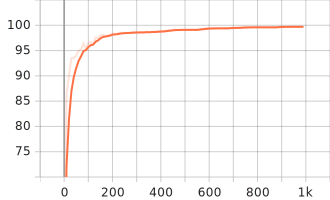
\includegraphics[width=.9\linewidth]{result_files/train_accuracy.png}
  \captionof{figure}{train accuracy best run}
  \label{fig:test1}
\end{minipage}%
\begin{minipage}{.5\textwidth}
  \centering
  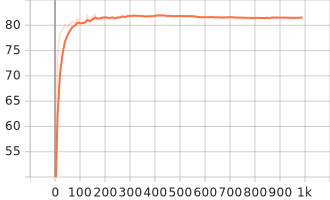
\includegraphics[width=.9\linewidth]{result_files/test_accuracy.png}
  \captionof{figure}{test accuracy best run}
  \label{fig:test2}
\end{minipage}
\end{figure}

700 epochs were necessary to achieve top performance

\begin{figure}
\centering
\begin{minipage}{.5\textwidth}
  \centering
  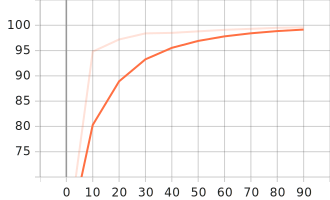
\includegraphics[width=.9\linewidth]{result_files/train_accuracy_2.png}
  \captionof{figure}{train accuracy second best run}
\end{minipage}%
\begin{minipage}{.5\textwidth}
  \centering
  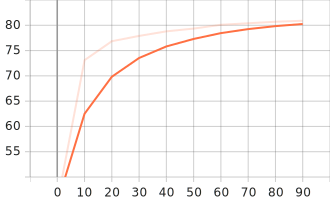
\includegraphics[width=.9\linewidth]{result_files/test_accuracy_2.png}
  \captionof{figure}{test accuracy second best run}

\end{minipage}
\end{figure}

all epochs were necessary to achieve top performance

\subsection{MSE vs CE}
MSE converges fast and has the highest test accuracy. 
\begin{figure}
\centering
\begin{minipage}{.5\textwidth}
  \centering
  \includegraphics[width=.9\linewidth]{result_files/accuracy_ce.png}
  \captionof{figure}{CE}
\end{minipage}%
\begin{minipage}{.5\textwidth}
  \centering
  \includegraphics[width=.9\linewidth]{result_files/accuracy_mse.png}
  \captionof{figure}{MSE}

\end{minipage}
\end{figure}



\end{document}